\documentclass[a4paper, fontsize=11pt]{scrartcl}

% Setup document
% tikz for graphics
\usepackage{enumitem}
\usepackage{amssymb}
\usepackage{tikz}
\usetikzlibrary{shapes, arrows.meta, positioning, calc, fit, shapes.geometric, shapes.multipart, shapes.arrows, decorations.pathreplacing}

% Import Eidesstattliche Erklärung
\usepackage{pdfpages}
% Import graphics and wrap them
\usepackage{graphicx}
\usepackage{wrapfig}
\usepackage{float}

% Localization
\usepackage[utf8]{inputenc}
\usepackage[T1]{fontenc}
\usepackage[ngerman]{babel}
\usepackage{csquotes}

% Bibliography
\usepackage[backend=biber, style=alphabetic, bibstyle=alphabetic, citestyle=alphabetic]{biblatex}

% Clickable table of contents
\usepackage{hyperref}
\usepackage[ngerman]{cleveref}

% Page formatting
\usepackage[automark]{scrlayer-scrpage}
\usepackage{typearea}
\usepackage{microtype}

% Better tables
\usepackage{tabularray}
\usepackage{booktabs}

% Develop Packages
\usepackage{blindtext}
% Variables
\newcommand{\vorname}{Lukas}
\newcommand{\nachname}{Szimtenings}
\newcommand{\matr}{Matr.-Nr.\ 3217694}
\newcommand{\uni}{FH Aachen}
\newcommand{\studiengang}{Angewandte Mathematik und Informatik}
\newcommand{\modul}{5. Semester 952006 (Aachen)}
\newcommand{\erstpruefer}{Alexander Voß}
\newcommand{\zweitpruefer}{Raphael Majeed}
\newcommand{\subtitel}{ Verteilte Ausführung von in konjunktiver Normalform spezifizierten Machbarkeitsabfragen in medizinischen Datenintegrationszentren }
\newcommand{\titel}{- Seminararbeit -}
\newcommand{\location}{Aachen}
\newcommand{\abteilung}{Abteilung: Research Infrastructure}
\newcommand{\abteilungabkuerzung}{RI}

%images
\newcommand{\uklogo}{
    \includegraphics[scale=0.5]{res/logo-uniklinik-rwth-aachen}
    \includegraphics[scale=0.6]{res/imi_sublogo}
}

\newcommand{\ukimilogo}{\includegraphics[scale=0.16]{res/imilogo}}
% command for wrapfigure -> more than one figure per paragraph
\newcommand*{\invisiblepar}{{\setlength{\parfillskip}{0pt}\par}\vskip-\parskip\noindent\ignorespaces}
% Metadata
\title{\titel}
\author{\vorname{} \nachname}
\date{\today{}, \location}

%%%%%%%%%%%%%%%%%%%%%%%%%%%%%%%%%%%%%%%%%%%%
%% Structure of the average document page %%
%%%%%%%%%%%%%%%%%%%%%%%%%%%%%%%%%%%%%%%%%%%%

\clearpairofpagestyles{}

% Footer
\ifoot[]{\itclogosmall}
\cfoot[]{\abteilungabkuerzung}
\ofoot[]{\pagemark}

% Header
\ihead[]{\vorname{} \nachname}
\chead[]{\titel}
\ohead[]{\matr}

% Separator between header/footer and page content
\KOMAoptions{headsepline=1pt}
\KOMAoptions{footsepline=1pt}

% newline after paragraph and subparagaph
\RedeclareSectionCommands[
  afterskip=1sp
]{paragraph,subparagraph}

\addbibresource{Seminararbeit.bib}

\RedeclareSectionCommands[
  afterskip=1sp
]{paragraph,subparagraph}

\begin{document}
%% Prefix %%
\input{sections/title_page.tex}
% Einbinden der Eidesstattlichen Erklärung
\includepdf{res/EidesstattlicheErklaerung.pdf}
\tableofcontents
\newpage

%% Hauptteil %%
% Seitenzahlen beginnen ab hier
\pagenumbering{arabic}

\section{Zusammenfassung und Ausblick}\label{sec:zusammenfassung}
   \subsection{Zusammenfassung der Ergebnisse}\label{subsec:zusammenfassung}

\section{Zusammenfassung und Ausblick}\label{sec:zusammenfassung}
   \subsection{Zusammenfassung der Ergebnisse}\label{subsec:zusammenfassung}

\input{sections/methodik.tex}

\section{Prozessbeschreibung}

Diese Prozessbeschreibung basiert auf dem Interview mit einem Mitarbeiter des Identity Management Teams (IDM) derjenigen Organisation, welche den IdP betreibt und die Metadaten der Serviceprovider (SP) verwaltet.\\
Der Prozess umfasst die Verwaltung von externen und internen Datenquellen, die Kommunikation mit den Service Providern und die Pflege von Metadaten in einem Git-Repository.

\subsection{Ziele und Anforderungen des Prozesses}

Das Hauptziel des Prozesses ist die effektive Verwaltung von Metadaten für Serviceprovider. Dazu gehören:

\begin{itemize}
  \item Die Sammlung und Dokumentation von Informationen zu den Service Providern
  \item Die Prüfung, Aktualisierung und Validierung von Metadaten
  \item Die Kommunikation von Änderungen an relevante Parteien
  \item Die Sicherstellung der korrekten Konfiguration der IdP Server
\end{itemize}

\subsection{Prozesse}

\subsubsection{Neuen Provider eintragen}

\begin{enumerate}
  \item Der SP-Betreiber erstellt beim ITC Servicedesk ein Ticket per E-Mail.
  \item Das Ticket geht an die IDM-Gruppe, die das Ticket auf Informationen prüft.
  \item Die IDM-Gruppe erstellt ein Request-for-Change (RFC)-Dokument (PDF) zur Sammlung und Dokumentation der Informationen.
  \item Das RFC-Dokument wird an den SP gesendet, um evtl.\ fehlende Informationen zu ergänzen und den RFC zu validieren.
  \item Die IDM-Gruppe prüft das RFC-Dokument auf Vollständigkeit und Korrektheit der Informationen.
  \item Bei Fehlern, Rückfragen oder Anpassungen wird wieder mit dem SP kommuniziert.
  \item Während das RFC noch geprüft wird, erhält der SP Zugriff zum Testsystem.
  \item Die IDM-Gruppe prüft den XML-Metadatensatz, der aus dem RFC hervorgeht mit einem linter auf Syntaxfehler.
  \item Die IDM-Gruppe fügt den XML-Metadatensatz in das Git-Repository ein.
  \item Eine zweite Datei mit Attributfiltern wird aus den angeforderten Attributen im RFC manuell erstellt und in einem anderen Git-Repository gespeichert.
\end{enumerate}

\subsubsection{Bestehende Provider anpassen}

\begin{enumerate}
  \item Der SP-Betreiber identifiziert die Notwendigkeit, die Metadaten eines bestehenden SP zu aktualisieren.
  \item Der SP-Betreiber sendet die aktualisierten Informationen an die IDM-Gruppe, die diese überprüft.
  \item Bei Fehlern, Rückfragen oder Anpassungen wird wieder mit dem SP kommuniziert.
  \item Die IDM-Gruppe verwendet einen XML-Linter, um die XML-Metadaten auf Syntaxfehler zu prüfen.
  \item Die IDM-Gruppe aktualisiert den XML-Metadatensatz und die Attributfilter-Datei in den Git-Repositories entsprechend der aktualisierten Informationen.
  \item Die IDM-Gruppe prüft manuell, ob das Login bei dem Serviceprovider funktioniert.
\end{enumerate}

\subsubsection{Metadatenänderungen in der IdP-Konfiguration vornehmen}

\begin{enumerate}
  \item Die XML-Metadaten in den Git-Repositories werden regelmäßig auf Änderungen überprüft.
  \item Die XML-Dokumente werden automatisch zusammengeführt.
  \item Der Merge wird auf die IdP Server hochgeladen.
\end{enumerate}

\subsection{Kommunikation}
Die Kommunikation im Prozess erfolgt über verschiedene Kanäle:

\begin{itemize}
  \item E-Mail: Hauptkommunikationsmittel für den Austausch von Informationen und Dokumenten
  \item Ticketsystem: Zur initialen Kontaktaufnahme zwischen IDM-Gruppe und SP-Betreiber
\end{itemize}

\subsection{Zeitlicher Aufwand}

Der gesamte zeitliche Aufwand für den Prozess der Metadatenverwaltung kann je nach Komplexität des Falls und der Anzahl der Rückfragen und Diskussionen mit den Serviceprovider Betreibern variieren. 
In der Regel dauert der gesamte Prozess zwischen 3 und 5 Tagen, kann allerdings auch bei Entwicklerwechsel bis zu einem Monat dauern

Von dieser Gesamtdauer entfällt ein erheblicher Teil auf das Abwarten von Rückmeldungen der Serviceprovider Betreiber.
Die effektive Arbeitszeit, die für die Verwaltung der Metadaten benötigt wird, beträgt minimal 4 Arbeitsstunden, und lässt sich dabei in drei Hauptkomponenten unterteilen:

\paragraph{Kommunikation:}
Die Kommunikation zwischen Serviceprovider Betreibern und IDM Gruppe bei Rückfragen zu Attributen ist ein großer Teil des Prozesses.
Die Dauer dieser Kommunikation hängt unter anderem von der Anzahl der offenen Fragen, der Reaktionsgeschwindigkeit der SP-Anbieter, der von den SP-Anbietern geleisteten Vorarbeit und den angefragten Attributen ab. 
Der Zeitaufwand kann daher stark variieren, stellt jedoch in aller Regel einen großen Teil der effektiven Arbeitszeit dar.
\paragraph{Dokumentation}
Im trivialsten Fall fallen für die Dokumentation in Form des RFC 1-2 Stunden an, dies hängt aber wieder von der Komplexität des Falls ab. 
\paragraph{Eintragen, Anpassen und Validieren von Anbindungen:}
Der verbleibende Teil der effektiven Arbeitszeit wird für das eigentliche Eintragen und Anpassen der Anbindungen aufgewendet.
Dies beinhaltet das erstellen des Attributfilters, das einholen der Metadaten von dem SP und das Deployment über die Git-Repositories.
Der Zeitaufwand für diese Aktivitäten kann ebenfalls variieren, allerdings nicht so sehr wie die für die Kommunikation aufgewendete Zeit.


Zusammenfassend kann der Prozess der Metadatenverwaltung in Bezug auf den zeitlichen Aufwand in effektive Arbeitszeit und Wartezeit auf Daten oder Rückmeldungen unterteilt werden. 
Die effektive Arbeitszeit wird hauptsächlich für Kommunikation, Dokumentation und Verwaltungsaufgaben aufgewendet.

\newpage
\subsection{Modell}
Die Abbildung~\ref{fig:service-provider-erstellung} modelliert den Prozess zur Eintragung eines neuen Service Providers.
% Importiere res/Service Provider Erstellung.png
\begin{figure}[H]
  \centering
  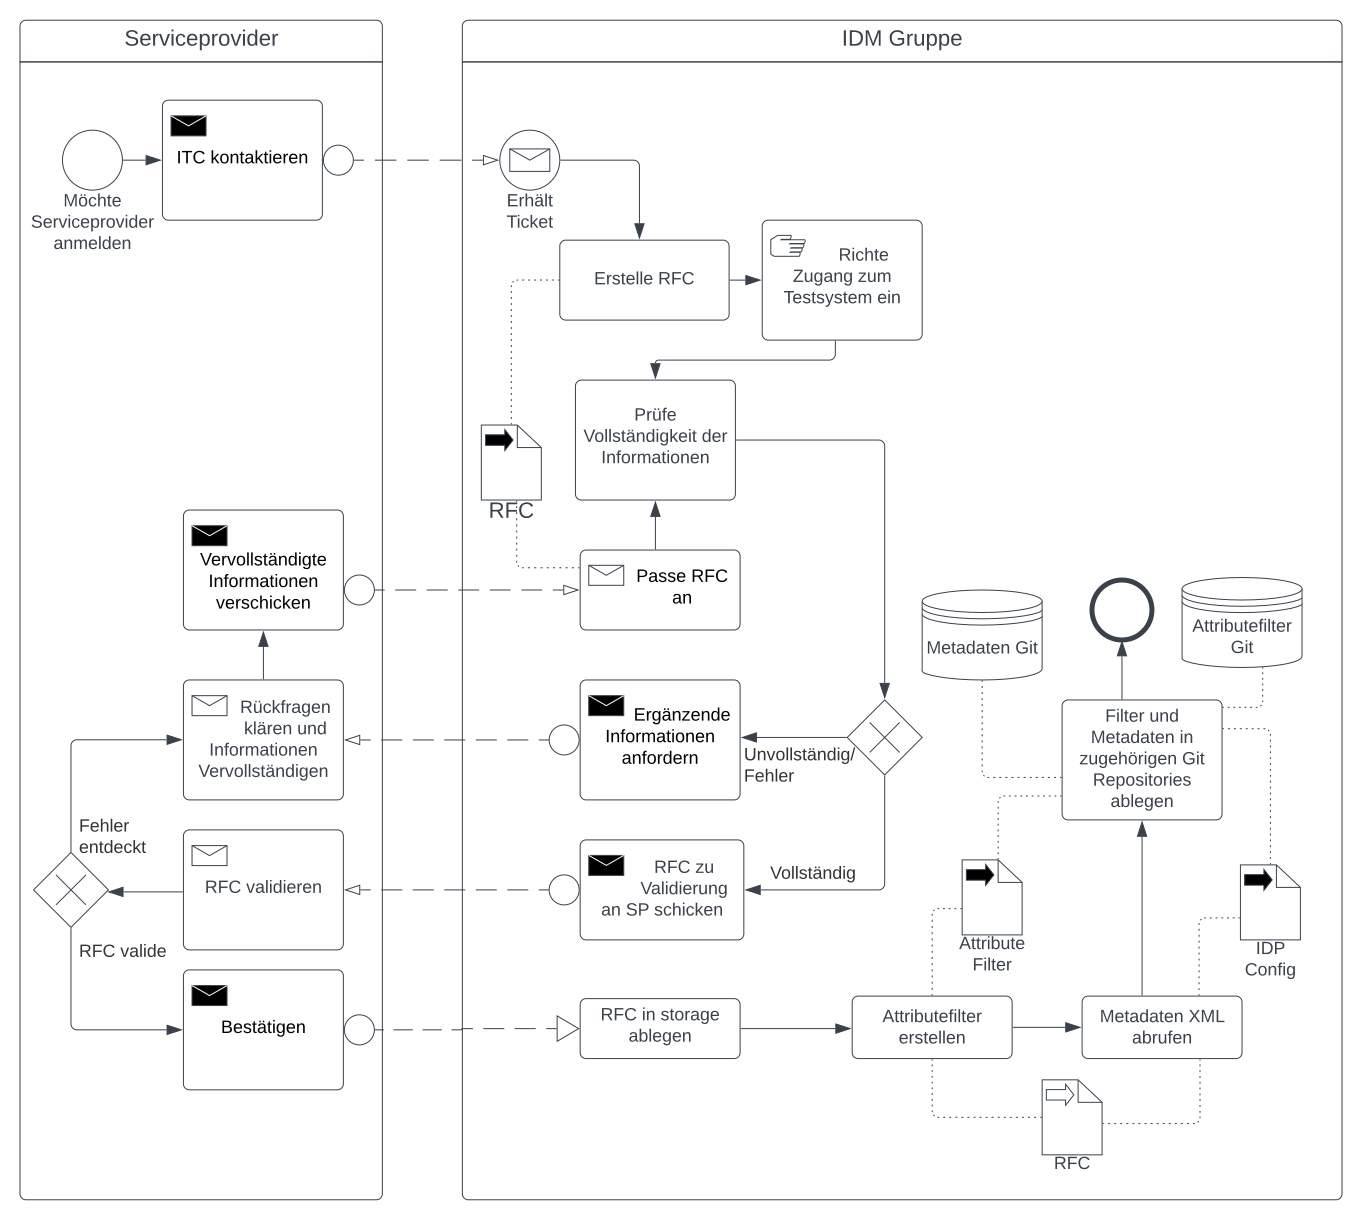
\includegraphics[width=0.8\textwidth]{res/Service Provider Erstellung.png}
  \caption{Prozess zur Eintragung eines neuen Service Providers}\label{fig:service-provider-erstellung}
\end{figure}

Die Abbildung~\ref{fig:service-provider-anpassung} modelliert den Prozess zur Anpassung eines bestehenden Service Providers. Es lässt sich feststellen, dass diese sich nur geringfügig von dem Prozess zur Eintragung eines neuen Service Providers unterscheidet.
% Importiere res/Service Provider Anpassung.png
\begin{figure}[H]
  \centering
  \includegraphics[width=0.8\textwidth]{res/Serviceprovider Anpassung.png}
  \caption{Prozess zur Anpassung eines bestehenden Service Providers}\label{fig:service-provider-anpassung}
\end{figure}



\section{Ergebnisse und Diskussion}\label{sec:results}

\subsection{Prozessanalyse}\label{subsec:prozessanalyse-results}
Die aktuelle Prozessanalyse zeigt verschiedene Schritte zur Verwaltung von Metadaten und Service Providern (SP) im Identity Management (IDM). 
Dabei werden Datenquellen, Metadaten, Benutzer- und Provider-Verwaltung sowie Kommunikation und Validierung von Metadatenänderungen behandelt.

\subsubsection{Probleme}
Die Analyse zeigt folgende Schwierigkeiten und Zeitaufwand bei der Metadatenverwaltung auf.


\paragraph{Inkonsistenzen zwischen RFC und effektiv verwendeten Metadaten}
Im aktuellen Prozess kann es zu Inkonsistenzen zwischen den im RFC-Dokument festgelegten Informationen und den tatsächlich verwendeten Metadaten kommen. 
Diese Diskrepanzen treten insbesonder dann auf, wenn geforderte Attribute sich während der Abgabe regelmäßig ändern.
Daneben tragen kurzfristig informell beantragte Änderungen zu Inkonsistenzen bei.

\paragraph{Zertifikatabläufe}
Ein weiteres Problem besteht darin, dass der Ablauf von Zertifikaten aktuell nicht geprüft wird. Der Shibboleth-Server geht dabei davon aus, dass alles Zertifikate gültig sind.\\
Dies ist zwar nicht sonderlich Sicherheitskritisch, allerdings dennoch ein unschöner Zustand.

\paragraph{Zeitkonsumierende Kommunikation mit Serviceprovider Betreibern}
Die Kommunikation mit den Serviceprovider Betreibern bei Rückfragen zu Attributen kann zeitintensiv sein.
Der gesamte Prozess dauert im Schnitt 3-5 Tage, wobei das Warten auf die Kommunikation einen erheblichen Anteil an der Gesamtdauer hat.
Mehr angeforderte Attribute führen dabei zu mehr Abstimmungsbedarf mit SP-Anbietern und damit zu einer stark erhöhten Dauer des Prozesses.

\paragraph{Karteileichen durch nicht existente Datenüberwachung}
Da keine Überwachung der existierenden Daten stattfindet und sich das Serviceprovider Administrationspersonal ändern kann, kann es zu Karteileichen kommen.
Dies bedeutet, dass einige Serviceprovider möglicherweise nicht mehr genutzt werden oder veraltet sind, aber weiterhin im System vorhanden sind.

\paragraph{Fehlende semantische Validierung der XML Metadaten}

Derzeit findet keine semantische Validierung der XML Metadaten statt.
Obwohl ein XML Linter verwendet wird, ist die Validierung mittels der Shibboleth XML Schema Definition (XSD) auf Dauer wünschenswert.
Die fehlende semantische Prüfung kann dazu führen, dass Fehler bei der Eintragung auftreten, und die Qualität der Metadaten beeinträchtigt wird.

\subsubsection{Verbesserungsvorschläge}
Die oben angeführten Probleme können durch die folgenden Verbesserungsvorschläge behoben oder gelindert werden.

\paragraph{Einführung eines Self-Service-Portals für Serviceprovider}
Um den zeitintensiven Kommunikationsaufwand mit Serviceprovider Betreibern zu reduzieren und die Effizienz des Prozesses zu erhöhen, könnte ein Self-Service-Portal implementiert werden.
Serviceprovider Betreiber könnten über dieses Portal eigenständig die benötigten Attribute anfordern und Änderungen an ihren Anbindungen vornehmen.
Dieses könnte das bisherige RFC-Dokument ersetzen und damit große Teile der Zeitaufwendigen Kommunikation mit der IDM-Gruppe übernehmen. Dies würde den Prozess aus Sicht der IDM Gruppe stark beschleunigen.

\paragraph{Automatische Überwachung und Validierung der Datenbestände}
Die Implementierung einer automatischen Überwachung und Validierung der Datenbestände könnte dazu beitragen, Karteileichen zu vermeiden.
Ein solches System könnte regelmäßig die Gültigkeit und Aktualität der Metadaten und Zertifikate überprüfen und bei Bedarf Warnungen oder Benachrichtigungen an die zuständigen Administratoren senden.
Kombiniert mit einem Self-Service-Portal welches die RFC-Dokumente ersetzt, würde das Problem der Inkonsistenzen damit gelöst und den manuellen Aufwand für die Prüfung und Aktualisierung der Datenbestände reduzieren.

\paragraph{Erweiterte semantische Validierung der XML Metadaten}
Die Einführung einer erweiterten semantischen Validierung der XML Metadaten mittels der Shibboleth XML Schema Definition (XSD) würde dazu beitragen, Fehler bei der Eintragung zu vermeiden und die Qualität der Metadaten zu verbessern.
Eine solche Validierung könnte automatisch im Rahmen der automatischen Überwachung der Datenbestände erfolgen und bei Bedarf entsprechende Korrekturmaßnahmen anstoßen.

\subsubsection{Diskussion}\label{subsubsec:prozessanalyse-discussion}
Der aktuelle Prozess zur Metadatenverwaltung und SP-Anbindung weist in einigen Bereichen Verbesserungspotenzial auf.
Durch die Einführung eines Self-Service-Portals könnte Kommunikation die aktuell einen großen Teil der für den Prozess benötigten Zeit in Anspruch nimmt reduziert werden.
Des weiteren könnte ein solches Portal die 
Durch Überwachungsmechanismen könnten Effizienz und Qualität des Prozesses gesteigert werden.

\subsection{Anforderungsanalyse}\label{subsec:anforderungsanalyse-results}
Auf Grundlage der Prozessanalyse ergeben sich die folgenden Anforderungen an ein System zur Verwaltung von Metadaten und Service Providern (SP) im Identity Management (IDM).

\subsubsection{Funktionale Anforderungen}\label{subsubsec:functional-requirements}
\paragraph{Antrag auf Ersteinrichtung stellen (SP):}
Noch nicht registrierte Serviceprovider Betreiber sollen die Möglichkeit haben, über die Plattform einen Antrag auf Ersteinrichtung ihres Services zu stellen.
Nachdem der Antrag eingereicht wurde, sollten die zuständigen Administratoren benachrichtigt werden, um den Antrag zu überprüfen, Rückfragen zu klären und im Anschluss entsprechend zu genehmigen oder abzulehnen. 
Über Genehmigung oder Ablehnung wird der Antragsteller benachrichtigt.

\paragraph{Antäge für Änderungen stellen (SP):}
Serviceprovider Betreiber dürfen keine direkten Änderungen an ihren Anbindungen vornehmen.
Stattdessen werden Anträge gestellt, die von Administratoren geprüft und entweder angenommen oder abgelehnt werden.

\paragraph{Attribute aus vorgegebener Liste auswählen (SP):}
Serviceprovider Betreiber sollten in der Lage sein, die benötigten Attribute aus einer vorgegebenen Liste auszuwählen.
Dies stellt sicher, dass nur gültige Attribute verwendet werden und die Konsistenz der Daten gewährleistet ist.

\paragraph{Zertifikatsverwaltung (SP):}
Serviceprovider Betreiber sollten in der Lage sein, ihre Zertifikate zu verwalten, einschließlich des Hochladens neuer Zertifikate zum ersetzen abgelaufener Zertifikate.
Das System muss dabei den aktuell existierenden Rollover Prozess umsetzen.

\paragraph{Metadatenvalidierung (SP):}
Serviceprovider Betreiber sollten durch das System unterstützt werden, um die Qualität und Konsistenz ihrer Metadaten zu gewährleisten.
Dies kann beispielsweise durch automatische Validierung der XML Metadaten mittels der Shibboleth XML Schema Definition (XSD) erfolgen.

\paragraph{Generierung von AttributeFiltern (IdP):}
Das System soll in der Lage sein aus den vom Serviceprovider ausgewählten Attributen AttributeFilter zu generieren, und damit die Wiederspruchsfreiheit der Daten sicher zu stellen.

\paragraph{Antragsverwaltung (IdP):}
Die Plattform sollte den Administratoren ermöglichen, aktuelle Anträge einzusehen und abzuarbeiten. Diese Anträge repräsentieren relevante Änderungen, die von Service Provider Betreibern angefordert wurden.
Administratoren sollten in der Lage sein, diese Anträge zu überprüfen, zu genehmigen oder abzulehnen und den Status der Anträge zu aktualisieren.
Die Antragsverwaltung trägt zur effizienten Kommunikation und Zusammenarbeit zwischen Identity Providern und Service Providern bei.

\paragraph{Übersichtsseite (IdP):}
Die Plattform sollte eine übersichtliche Liste aller Service Provider anzeigen, um den Administratoren einen schnellen und einfachen Zugriff auf Informationen und Einstellungen der einzelnen Service Provider zu ermöglichen.
Administratoren sollten in der Lage sein, die Übersichtsseite zu nutzen, um den Status und die Konfiguration von Service Providern einfach zu verwalten und zu überwachen.

\subsubsection{Nicht-funktionale Anforderungen}\label{subsubsec:non-functional-requirements}

\paragraph{Design-Konsistenz:}
Die Plattform soll dem Design von bereits bestehenden Plattformen folgen, um eine konsistente Benutzererfahrung und ein einheitliches Erscheinungsbild zu gewährleisten. 
Dies erleichtert die Integration der neuen Plattform in die bestehende Systemlandschaft und verbessert die Benutzerakzeptanz.

\paragraph{Technologie und Interoperabilität:}
Die Plattform muss in Apache Wicket entwickelt werden, um die Interoperabilität mit bestehenden Systemen sicherzustellen und die Wartbarkeit durch vorhandenes Personal zu ermöglichen.
Die Verwendung von Apache Wicket trägt dazu bei, dass die Plattform nahtlos in die bestehende Infrastruktur integriert werden kann und die Lernkurve im Falle einer Übergabe gering ist.


\section{Zusammenfassung und Ausblick}\label{sec:summary}
\subsection{Zusammenfassung}\label{subsec:summary}
In dieser Seminararbeit liegt der Schwerpunkt auf der Analyse des aktuellen Prozesses zur Verwaltung der Service Provider durch die Identity Management Gruppe, basierend auf einem Interview mit dem Identity Provider (IdP)-Betreiber.
Ziel der Arbeit ist es, Schwachstellen in der Metadatenverwaltung zu identifizieren und Verbesserungsvorschläge vorzuschlagen, um die Effizienz und Qualität des Prozesses zu erhöhen.

Die Analyse zeigt folgende Schwierigkeiten und Probleme auf:

\begin{enumerate}
    \item Inkonsistenzen zwischen RFC und effektiv verwendeten Metadaten: Diskrepanzen können auftreten, wenn sich geforderte Attribute während der Abgabe ändern oder informell beantragte Änderungen kurzfristig eintreten.
    \item Zeitkonsumierende Kommunikation mit Serviceprovider Betreibern: Der gesamte Prozess dauert im Schnitt 3--5 Tage, wobei das Warten auf die Kommunikation einen erheblichen Anteil an der Gesamtdauer hat.
    \item Karteileichen durch nicht existente Datenüberwachung: Da keine Überwachung der existierenden Daten stattfindet, können veraltete oder nicht mehr genutzte Serviceprovider im System verbleiben.
    \item Fehlende semantische Validierung der XML Metadaten: Die fehlende Validierung mittels der Shibboleth XML Schema Definition (XSD) kann zu Fehlern bei der Eintragung und einer Beeinträchtigung der Metadatenqualität führen.
\end{enumerate}

Um diese Schwachstellen zu beheben, wurden Verbesserungsvorschläge erarbeitet:

\begin{enumerate}
    \item Einführung eines Self-Service-Portals für Serviceprovider: Dadurch können Serviceprovider Betreiber eigenständig die benötigten Attribute anfordern und Änderungen an ihren Anbindungen vornehmen, was den Kommunikationsaufwand und die Prozessdauer reduziert.
    \item Automatische Überwachung und Validierung der Datenbestände: Ein solches System kann die Gültigkeit und Aktualität der Metadaten und Zertifikate überprüfen und bei Bedarf Warnungen oder Benachrichtigungen an die zuständigen Administratoren senden, wodurch der manuelle Aufwand für die Prüfung und Aktualisierung der Datenbestände reduziert wird.
    \item Erweiterte semantische Validierung der XML-Metadaten: Durch die Verwendung der Shibboleth XML Schema Definition (XSD) können Fehler bei der Eintragung vermieden und die Qualität der Metadaten verbessert werden.
\end{enumerate}

\subsection{Ausblick}\label{subsec:outlook}
Die in dieser Seminararbeit präsentierten Verbesserungsvorschläge stellen einen fundierten Ausgangspunkt für die Optimierung des Prozesses zur Verwaltung von Identity Providern und Service Providern dar.
Im Folgenden werden potenzielle weiterführende Forschungsansätze und Entwicklungen skizziert, um die Zusammenarbeit zwischen IdPs und SPs zu intensivieren und den Prozess effizienter zu gestalten.

Eine Folgearbeit könnte die Anforderungsanalyse weiter vertiefen und anschließend einen detaillierten Systementwurf für das Self-Service-Portal erstellen.
Der Systementwurf sollte die Architektur, Schnittstellen, Datenstrukturen sowie Sicherheitsanforderungen des Portals präzise darstellen.

Als weiterer Forschungsschritt könnten die Auswirkungen der implementierten Verbesserungen auf die Effizienz und Qualität des Prozesses untersucht werden.
Empirische Studien, die den Zeitaufwand, die Fehleranfälligkeit und die Zufriedenheit der Benutzer vor und nach der Implementierung der Verbesserungen vergleichen, könnten wertvolle Erkenntnisse für die Evaluation der vorgeschlagenen Lösungen liefern.
Basierend auf diesen Ergebnissen könnten gegebenenfalls zusätzliche Anpassungen und Optimierungen vorgenommen werden, um den Gesamtprozess weiter zu verbessern.

%% Suffix %%
\newpage

% Bibliographie
\pagenumbering{Roman}
\printbibliography{}
% Abbildungsverzeichnis
\listoffigures
\end{document}